

\tikzset{every picture/.style={line width=0.75pt}} %set default line width to 0.75pt        

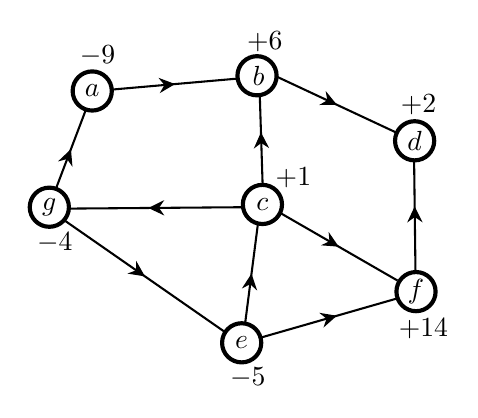
\begin{tikzpicture}[x=0.5pt,y=0.5pt,yscale=-1,xscale=1]
%uncomment if require: \path (0,271); %set diagram left start at 0, and has height of 271

%Straight Lines [id:da5212458340621946] 
\draw [color={rgb, 255:red, 0; green, 0; blue, 0 }  ,draw opacity=1 ][line width=0.75]    (72.5,45) -- (164,37) ;
\draw [shift={(118.25,41)}, rotate = 175] [fill={rgb, 255:red, 0; green, 0; blue, 0 }  ,fill opacity=1 ][line width=0.08]  [draw opacity=0] (11.61,-5.58) -- (0,0) -- (11.61,5.58) -- (7.71,0) -- cycle    ;
%Straight Lines [id:da5107871061349898] 
\draw [color={rgb, 255:red, 0; green, 0; blue, 0 }  ,draw opacity=1 ][line width=0.75]    (278,76) -- (192.5,36) ;
\draw [shift={(235.25,56)}, rotate = 205.07] [fill={rgb, 255:red, 0; green, 0; blue, 0 }  ,fill opacity=1 ][line width=0.08]  [draw opacity=0] (11.61,-5.58) -- (0,0) -- (11.61,5.58) -- (7.71,0) -- cycle    ;
%Straight Lines [id:da33373699050559813] 
\draw [color={rgb, 255:red, 0; green, 0; blue, 0 }  ,draw opacity=1 ][line width=0.75]    (291,96) -- (292,177) ;
\draw [shift={(291.41,129.4)}, rotate = 89.29] [fill={rgb, 255:red, 0; green, 0; blue, 0 }  ,fill opacity=1 ][line width=0.08]  [draw opacity=0] (11.61,-5.58) -- (0,0) -- (11.61,5.58) -- (7.71,0) -- cycle    ;
%Straight Lines [id:da41415742704032066] 
\draw [color={rgb, 255:red, 0; green, 0; blue, 0 }  ,draw opacity=1 ][line width=0.75]    (181,224) -- (278.5,196) ;
\draw [shift={(235.13,208.45)}, rotate = 163.98] [fill={rgb, 255:red, 0; green, 0; blue, 0 }  ,fill opacity=1 ][line width=0.08]  [draw opacity=0] (11.61,-5.58) -- (0,0) -- (11.61,5.58) -- (7.71,0) -- cycle    ;
%Straight Lines [id:da5297018905877636] 
\draw [color={rgb, 255:red, 0; green, 0; blue, 0 }  ,draw opacity=1 ][line width=0.75]    (181.5,113) -- (179.5,50) ;
\draw [shift={(180.32,75.9)}, rotate = 88.18] [fill={rgb, 255:red, 0; green, 0; blue, 0 }  ,fill opacity=1 ][line width=0.08]  [draw opacity=0] (11.61,-5.58) -- (0,0) -- (11.61,5.58) -- (7.71,0) -- cycle    ;
%Straight Lines [id:da9441285731905983] 
\draw [color={rgb, 255:red, 0; green, 0; blue, 0 }  ,draw opacity=1 ][line width=0.75]    (54,59) -- (32,117) ;
\draw [shift={(43,88)}, rotate = 110.77] [fill={rgb, 255:red, 0; green, 0; blue, 0 }  ,fill opacity=1 ][line width=0.08]  [draw opacity=0] (11.61,-5.58) -- (0,0) -- (11.61,5.58) -- (7.71,0) -- cycle    ;
%Straight Lines [id:da3078405450216426] 
\draw [color={rgb, 255:red, 0; green, 0; blue, 0 }  ,draw opacity=1 ][line width=0.75]    (167,130) -- (42,131) ;
\draw [shift={(98.9,130.54)}, rotate = 359.54] [fill={rgb, 255:red, 0; green, 0; blue, 0 }  ,fill opacity=1 ][line width=0.08]  [draw opacity=0] (11.61,-5.58) -- (0,0) -- (11.61,5.58) -- (7.71,0) -- cycle    ;
%Straight Lines [id:da3541622648157198] 
\draw [color={rgb, 255:red, 0; green, 0; blue, 0 }  ,draw opacity=1 ][line width=0.75]    (154,220) -- (39,140) ;
\draw [shift={(96.5,180)}, rotate = 214.82] [fill={rgb, 255:red, 0; green, 0; blue, 0 }  ,fill opacity=1 ][line width=0.08]  [draw opacity=0] (11.61,-5.58) -- (0,0) -- (11.61,5.58) -- (7.71,0) -- cycle    ;
%Straight Lines [id:da720688848918495] 
\draw [color={rgb, 255:red, 0; green, 0; blue, 0 }  ,draw opacity=1 ][line width=0.75]    (279,183) -- (194,134) ;
\draw [shift={(236.5,158.5)}, rotate = 209.96] [fill={rgb, 255:red, 0; green, 0; blue, 0 }  ,fill opacity=1 ][line width=0.08]  [draw opacity=0] (11.61,-5.58) -- (0,0) -- (11.61,5.58) -- (7.71,0) -- cycle    ;
%Straight Lines [id:da4466024070919401] 
\draw [color={rgb, 255:red, 0; green, 0; blue, 0 }  ,draw opacity=1 ][line width=0.75]    (178,143) -- (169,213) ;
\draw [shift={(173.5,178)}, rotate = 97.33] [fill={rgb, 255:red, 0; green, 0; blue, 0 }  ,fill opacity=1 ][line width=0.08]  [draw opacity=0] (11.61,-5.58) -- (0,0) -- (11.61,5.58) -- (7.71,0) -- cycle    ;

% Text Node
\draw (47.24,11.06) node [anchor=north west][inner sep=0.75pt]   [align=left] {$\displaystyle -9$};
% Text Node
\draw  [line width=1.5]   (27.38, 130) circle [x radius= 14.15, y radius= 14.15]   ;
\draw (27.38,130) node   [align=left] {$\displaystyle g$};
% Text Node
\draw  [line width=1.5]   (58.38, 46) circle [x radius= 14.15, y radius= 14.15]   ;
\draw (58.38,46) node   [align=left] {$\displaystyle a$};
% Text Node
\draw  [line width=1.5]   (177.48, 35) circle [x radius= 14.15, y radius= 14.15]   ;
\draw (171.98,35) node [anchor=west] [inner sep=0.75pt]   [align=left] {$\displaystyle b$};
% Text Node
\draw  [line width=1.5]   (181.38, 128) circle [x radius= 14.15, y radius= 14.15]   ;
\draw (181.38,128) node   [align=left] {$\displaystyle c$};
% Text Node
\draw  [line width=1.5]   (291.38, 82) circle [x radius= 14.15, y radius= 14.15]   ;
\draw (291.38,82) node   [align=left] {$\displaystyle d$};
% Text Node
\draw  [line width=1.5]   (166.38, 228) circle [x radius= 14.15, y radius= 14.15]   ;
\draw (166.38,228) node   [align=left] {$\displaystyle e$};
% Text Node
\draw  [line width=1.5]   (292.38, 191) circle [x radius= 14.15, y radius= 14.15]   ;
\draw (292.38,191) node   [align=left] {$\displaystyle f$};
% Text Node
\draw (16.24,146.06) node [anchor=north west][inner sep=0.75pt]   [align=left] {$\displaystyle -4$};
% Text Node
\draw (279.24,46.06) node [anchor=north west][inner sep=0.75pt]   [align=left] {$\displaystyle +2$};
% Text Node
\draw (155.75,244) node [anchor=north west][inner sep=0.75pt]   [align=left] {$\displaystyle -5$};
% Text Node
\draw (168,1) node [anchor=north west][inner sep=0.75pt]   [align=left] {$\displaystyle +6$};
% Text Node
\draw (277.75,208) node [anchor=north west][inner sep=0.75pt]   [align=left] {$\displaystyle +14$};
% Text Node
\draw (188.75,99) node [anchor=north west][inner sep=0.75pt]   [align=left] {$\displaystyle +1$};


\end{tikzpicture}

